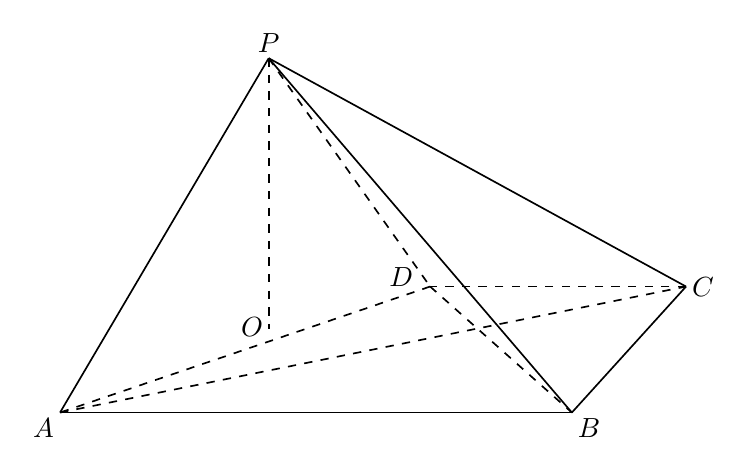
\begin{tikzpicture}[x=1cm,y=1cm,font=\normalsize,
  geometry edge/.style={solid,line width=.6pt},
  geometry label/.style={font=\normalsize,inner sep=2pt}]
\coordinate (P) at (-0.85,4.5);
\coordinate (A) at (-3.5,0);
\coordinate (B) at (3,0);
\coordinate (D) at (1.2,1.6);
\coordinate (C) at (4.45,1.6);
\coordinate (O) at (-0.85,1.066666667);
% base outline
\draw[geometry edge] (A)--(B);
\draw[geometry edge] (B)--(C);
\draw[geometry edge,dashed] (C)--(D);
\draw[geometry edge,dashed] (D)--(A);
% base diagonals through O
\draw[geometry edge,dashed] (A)--(C);
\draw[geometry edge,dashed] (D)--(B);
% lateral edges
\draw[geometry edge] (P)--(A);
\draw[geometry edge] (P)--(B);
\draw[geometry edge] (P)--(C);
\draw[geometry edge,dashed] (P)--(D);
\draw[geometry edge,dashed] (P)--(O);
\node[geometry label,above] at (P) {$P$};
\node[geometry label,below left] at (A) {$A$};
\node[geometry label,below right] at (B) {$B$};
\node[geometry label,above left,xshift=-4.00bp,yshift=-2.00bp] at (D) {$D$};
\node[geometry label,right] at (C) {$C$};
\node[geometry label,below,xshift=-6.00bp,yshift=6.00bp] at (O) {$O$};
\end{tikzpicture}
